\documentclass[12pt]{article}
\usepackage[margin=1in]{geometry}
\usepackage{amsmath}
\usepackage{amssymb}
\usepackage{graphicx}
\usepackage{hyperref}
\usepackage{natbib}
\usepackage{float}
\usepackage{algorithm}
\usepackage{algorithmic}
\usepackage{xcolor}
\usepackage{tikz}
\usepackage{booktabs}

\title{Modeling Information Spread and Containment Using Reinforcement Learning Agents}
\author{Axel Kerbec}
\date{\today}

\begin{document}

\maketitle

\begin{abstract}
This paper presents a multi-agent reinforcement learning model for the spread and containment of information in social networks. Two competing agents, a spreader and a healer, operate in a network environment where they learn optimal strategies to either propagate or limit the spread of information. The model builds on epidemic modeling concepts but extends them to incorporate strategic decision-making by intelligent agents. We evaluate our approach across different network topologies and identify the critical factors that influence information diffusion dynamics. Results demonstrate that agent-based reinforcement learning can effectively model the competitive dynamics of information spread and reveal insights about optimal intervention strategies for misinformation containment.
\end{abstract}

\section{Introduction}

Information spreads through social networks in ways that parallel epidemiological processes, where ideas, beliefs, or misinformation can "infect" individuals through social interactions. The rapid growth of social media platforms has accelerated both the diffusion of information and the potential for misinformation to spread unchecked. Understanding how information propagates through networks and identifying effective strategies for either promoting valuable information or containing harmful misinformation has become a critical challenge.

Traditional approaches to modeling information diffusion have relied on epidemic models like SIR (Susceptible-Infected-Recovered) or SIS (Susceptible-Infected-Susceptible), which treat information spread as a stochastic process with fixed transition probabilities. However, these models often fail to capture the strategic nature of information diffusion in real-world scenarios, where both the spread and containment of information may be driven by intelligent actors with competing objectives.

Recent advances in reinforcement learning (RL) have opened new avenues for modeling complex, strategic interactions in network environments. RL approaches enable the modeling of agents that can learn and adapt their strategies based on feedback from the environment \citep{sutton2018reinforcement}, making them well-suited for capturing the dynamic nature of information diffusion processes.

In this paper, we present a multi-agent reinforcement learning model for information spread and containment in social networks. Our model features two competing agents:

\begin{itemize}
    \item Agent A (Spreader): Aims to maximize the spread of information across the network
    \item Agent B (Healer): Aims to contain or reduce the spread of information
\end{itemize}

These agents operate within a network environment where nodes represent individuals who can be either susceptible to or infected by information. The agents learn optimal strategies for selecting nodes to either spread or contain information, considering factors such as network topology, node states, and the evolving dynamics of the diffusion process.

Through this approach, we hope to address the following research questions:

\begin{enumerate}
    \item How do reinforcement learning agents adapt their strategies in response to different network topologies and diffusion parameters? How do those strategies differ from expectations? 
    \item What network characteristics most significantly impact the effectiveness of spreading or containing information?
    \item How does the balance between spreading and healing capabilities affect the equilibrium state of information diffusion?
\end{enumerate}

Our study contributes to the growing body of literature on computational approaches to misinformation management by providing insights into the strategic dynamics of information spread and containment. The findings from our model can inform the development of more effective interventions for promoting beneficial information or limiting the spread of harmful misinformation in social networks.

\section{Related Work}

\subsection{Information Diffusion Models}

Traditional information diffusion models have largely built upon epidemic modeling frameworks. The two most prominent approaches are Independent Cascade (IC) models and Linear Threshold (LT) models. In IC models, each newly infected node has a single opportunity to infect each of its neighbors with a specified probability. LT models, on the other hand, assume that nodes become infected when the combined influence from their infected neighbors exceeds a certain threshold.

While these models have provided valuable insights into diffusion dynamics, they typically assume fixed propagation probabilities and do not account for strategic decision-making by the entities spreading or containing information.

Recent advances in reinforcement learning have enabled more sophisticated approaches to modeling decision-making processes in network environments. \citet{he2022reinforcement} proposed a reinforcement learning-based rumor blocking approach for directed social networks. \citet{chen2019reinforcement} applied deep Q-networks to the problem of maximizing information diffusion in social networks.

Multi-agent reinforcement learning (MARL) has emerged as a powerful framework for modeling strategic interactions between multiple decision-makers. \citet{qipeng2021influence} applied MARL to model influence maximization under competitive activation models, where multiple agents compete to spread their information through a network. This approach enables the modeling of complex, adaptive strategies that emerge from the interaction between competing agents.

Our work serves a proof-of-concept for a simulation environment and RL framework  where agents can continuously adapt their strategies based on the current state of the network and the actions of competing agents. By evaluating this framework across various network configurations, we provide insights into the factors that influence the dynamics of strategic information diffusion and containment. While there are many issues in our own model, it lays the foundation for further exploration and enhancement of policy choices to counter the spread of misinformation. 

This approach is very similar, and perhaps just a simplified version, of the methods presented in \citet{wijayanto2019effective}
\section{Methods}

\subsection{Model Description}

In this section, we describe our agent-based model for information spread and containment. The model consists of a network environment, two competing agents, and a set of rules governing their interactions.

\subsubsection{Environment}

The environment is a social network represented as a directed graph $G = (V, E)$, where $V$ is the set of nodes (individuals) and $E$ is the set of edges (social connections). Each edge $(u, v) \in E$ has a weight $w(u, v) \in [0, 1]$ representing the strength of influence that node $u$ has on node $v$.

Each node in the network can be in one of two states:
\begin{itemize}
    \item \textbf{Susceptible}: The node has not yet adopted the information.
    \item \textbf{Infected}: The node has adopted the information and can spread it to others.
\end{itemize}

Each node also has the following properties:
\begin{itemize}
    \item \textbf{Skepticism}: A value $s \in [0, 1]$ representing the node's resistance to adopting information. Higher skepticism reduces the probability of becoming infected.
    \item \textbf{Length of Infection}: For infected nodes, the number of time steps they have been in the infected state.
\end{itemize}

The network evolves over discrete time steps. At each time step, information can spread through the network according to interaction rules (mimicking epidemic dynamics), and agents can take actions to influence this process.

\subsubsection{Agents}

Our model features two competing agents:

\textbf{Agent A (Spreader)}: The objective of Agent A is to maximize the spread of information through the network. At each time step, Agent A selects a single node to "infect" with information.

\textbf{Agent B (Healer)}: The objective of Agent B is to contain or reduce the spread of information. At each time step, Agent B selects a node and a radius of influence. All nodes within the specified radius may recover from infection or become more resistant to infection.

The agents observe the current state of the network, including the state of each node, their properties, and various network features such as centrality measures and local infection rates. Based on these observations, the agents select actions to maximize their respective objectives.

\subsubsection{Interaction Rules}

Information spreads through the network according to the following rules:

\textbf{Infection}: An infected node $u$ can infect a susceptible neighbor $v$ with probability $p_{inf}(u, v) = p_0 \cdot (1 - s_v) \cdot w(u, v)$, where $p_0$ is the base infection probability, $s_v$ is the skepticism of node $v$, and $w(u, v)$ is the edge weight.

\textbf{Recovery}: An infected node can recover and become susceptible again with probability $p_{rec} = p_r / (1 + 0.1 \cdot d)$, where $p_r$ is the base recovery probability and $d$ is the duration of infection.

\textbf{Agent Actions}: 
\begin{itemize}
    \item Agent A selects a node $u$ to directly infect, bypassing the normal infection probability (though still affected by the node's skepticism).
    \item Agent B selects a node $v$ and a radius $r$. All nodes within distance $r$ of $v$ have:
    \begin{itemize}
        \item Increased probability of recovery (if infected)
        \item Reduced weight on incoming edges (reducing future infection probability)
        \item Increased skepticism (further reducing future infection probability)
    \end{itemize}

    Interventions of radius $r = 0$ (\textit{individual} intervention) can be carried out on nodes which are not infected. Such an intervention then only serves 
    to significantly slow down the spread of infection \textit{locally} by reducing all of the target node's incoming edge-weights. We term this a \emph{pre-emptive} 
    action by the Healing Agent. 

    Intervention of radius $r > 0$ work by slightly reducing 
    all edge weights within a $1$-step radiu of the selected node. We this a \emph{community-based} action by the Healing agent. 
\end{itemize}

\textbf{Network Dynamics}: As information spreads, the network itself evolves:
\begin{itemize}
    \item Edge weights between infected nodes increase slightly over time, representing reinforcement of shared beliefs.
    \item Edge weights to nodes that have recovered are significantly reduced, representing increased resistance to re-infection.
\end{itemize}

As will be spelled out later, siginificant choices that were made early have, unnforunately, limited our ability to extend this work to dynamic networks -- while our model certainly could accomodate such networks, it would require
a change in the learning architecture. We proceed to discuss 
implementation details. 

\subsection{Implementation}

\subsubsection{Network Generation}

We implement three types of network topologies for our experiments:

\begin{itemize}
    \item \textbf{Scale-Free Networks}: Generated using the Barabási–Albert model with preferential attachment, characterized by a power-law degree distribution. These networks have a few highly connected hubs and many nodes with few connections.
    
    \item \textbf{Small-World Networks}: Generated using the Watts-Strogatz model, characterized by high clustering and short average path lengths. These networks represent social structures with strong community clustering but occasional long-range connections.
    
    \item \textbf{Random Networks}: Generated using the Erdős–Rényi model, where edges are assigned randomly between nodes with a fixed probability. These networks serve as a baseline for comparison.
\end{itemize}

For each network type, we generate networks of 100 nodes with appropriate parameters to maintain similar average degree across types. Default parameters include:

\begin{table}[h]
\centering
\begin{tabular}{@{}lccc@{}}
\toprule
\textbf{Parameter} & \textbf{Scale-Free} & \textbf{Small-World} & \textbf{Random} \\
\midrule
Number of Nodes & 100 & 100 & 100 \\
Edge Parameter & $m=3$ & $k=8$ & $p=0.05$ \\
Initial Infection & 20\% & 10\% & 15\% \\
\bottomrule
\end{tabular}
\caption{Default network generation parameters}
\label{tab:network_params}
\end{table}

\subsubsection{Feature Extraction}

To enable agents to make informed decisions, we extract the following features from the network:

\begin{itemize}
    \item \textbf{Node State}: Whether a node is susceptible or infected.
    \item \textbf{Skepticism}: The node's resistance to infection.
    \item \textbf{Length of Infection}: How long a node has been infected.
    \item \textbf{Internal Influence}: A measure of how influential an infected node is within the subnetwork of infected nodes, calculated using eigenvector centrality.
    \item \textbf{Infection Pressure}: For susceptible nodes, the weighted sum of incoming influence from infected neighbors.
    \item \textbf{Spreading Potential}: For infected nodes, the weighted sum of outgoing influence to susceptible neighbors.
\end{itemize}

These features are normalized and organized into a feature matrix of shape (number of nodes, number of features) that serves as the state representation for the reinforcement learning agents.

\subsubsection{Reinforcement Learning Framework}

We implement our agents using the Proximal Policy Optimization (PPO) algorithm, a state-of-the-art policy gradient method known for its stability and sample efficiency. The agents are trained within a multi-agent environment using the following components:

\textbf{State Space}: The state space consists of the feature matrix described above, representing the current state of the network.

\textbf{Action Space}:
\begin{itemize}
    \item For Agent A: A discrete action space representing the node to infect.
    \item For Agent B: A composite action space consisting of a node selection and a radius selection (0, 1, or 2 steps from the selected node).
\end{itemize}

\textbf{Reward Functions}:
\begin{itemize}
    \item Agent A's reward: $R_A = 20 \cdot \Delta I + 2 \cdot I$, where $\Delta I$ is the change in infection rate and $I$ is the current infection rate.
    \item Agent B's reward: $R_B = -20 \cdot \Delta I + 2 \cdot (1 - I)$, inversely related to Agent A's reward.
\end{itemize}

\textbf{Network Architecture}: Each agent has a separate policy network implemented as a multi-layer perceptron with the following structure:
\begin{itemize}
    \item Input layer: Flattened feature matrix
    \item Hidden layers: Two hidden layers with 256 units each and ReLU activation
    \item Output layer: 
    \begin{itemize}
        \item For Agent A: Softmax output over all nodes
        \item For Agent B: Dual output with softmax over nodes and softmax over radius values
    \end{itemize}
\end{itemize}

\textbf{Training Procedure}: The agents are trained simultaneously using the following procedure:
\begin{enumerate}
    \item Initialize the network with a random seed of infected nodes
    \item For each time step:
    \begin{enumerate}
        \item Agents observe the current state and select actions
        \item Actions are executed in the environment
        \item Information propagates through the network
        \item Rewards are calculated and provided to the agents
        \item Agents update their policies using the PPO algorithm
    \end{enumerate}
    \item The episode ends when either all nodes are infected, no nodes are infected, or the maximum 
    number of steps per episode has been reached. 
\end{enumerate}

\subsection{Experimental Setup}

We conducted a series of experiments to evaluate the behavior of our model under different conditions and to answer our research questions. Our experimental setup consisted of three main components:

\subsubsection{Network Configurations}

We tested our model on three network types:
\begin{itemize}
    \item "Balanced" Scale-Free Network: A baseline configuration with moderate infection and recovery probabilities
    \item Small-World Network: A configuration with high clustering and short average path length
    \item "Viral" Scale-Free Network: A configuration with high infection probability and medium recovery probability
\end{itemize}

\subsubsection{Training Process}

For each network configuration, we trained the agents for 100 iterations, with each iteration consisting of multiple episodes. We used the following hyperparameters for training:
\begin{itemize}
    \item Batch size: 4000
    \item Learning rate: 5e-5
    \item Gamma (discount factor): 0.99
    \item Lambda (GAE parameter): 0.95
    \item Entropy coefficient: 0.2
\end{itemize}

\subsubsection{Evaluation Metrics}

We evaluated our model using the following metrics:
\begin{itemize}
    \item Infection rate: The proportion of nodes in the infected state
    \item Agent rewards: The cumulative rewards received by each agent
    \item Agent behavior patterns: Analysis of which nodes agents target and how they use their action capabilities
\end{itemize}

\subsubsection{Parameter Sweep}

To understand the impact of different parameters on the model's behavior, we conducted a parameter sweep across:
\begin{itemize}
    \item Infection probability: The base probability of infection spreading between nodes
    \item Recovery probability: The base probability of infected nodes recovering
    \item Initial infection density: The proportion of nodes initially infected
\end{itemize}

For each parameter combination, we ran the model with the trained agents and analyzed the resulting dynamics.

\section{Results}

\subsection{Baseline Simulation}
We first run a simulation on a small balanced network to serve as a baseline
for future results. 
\begin{figure}[h]
    \centering
    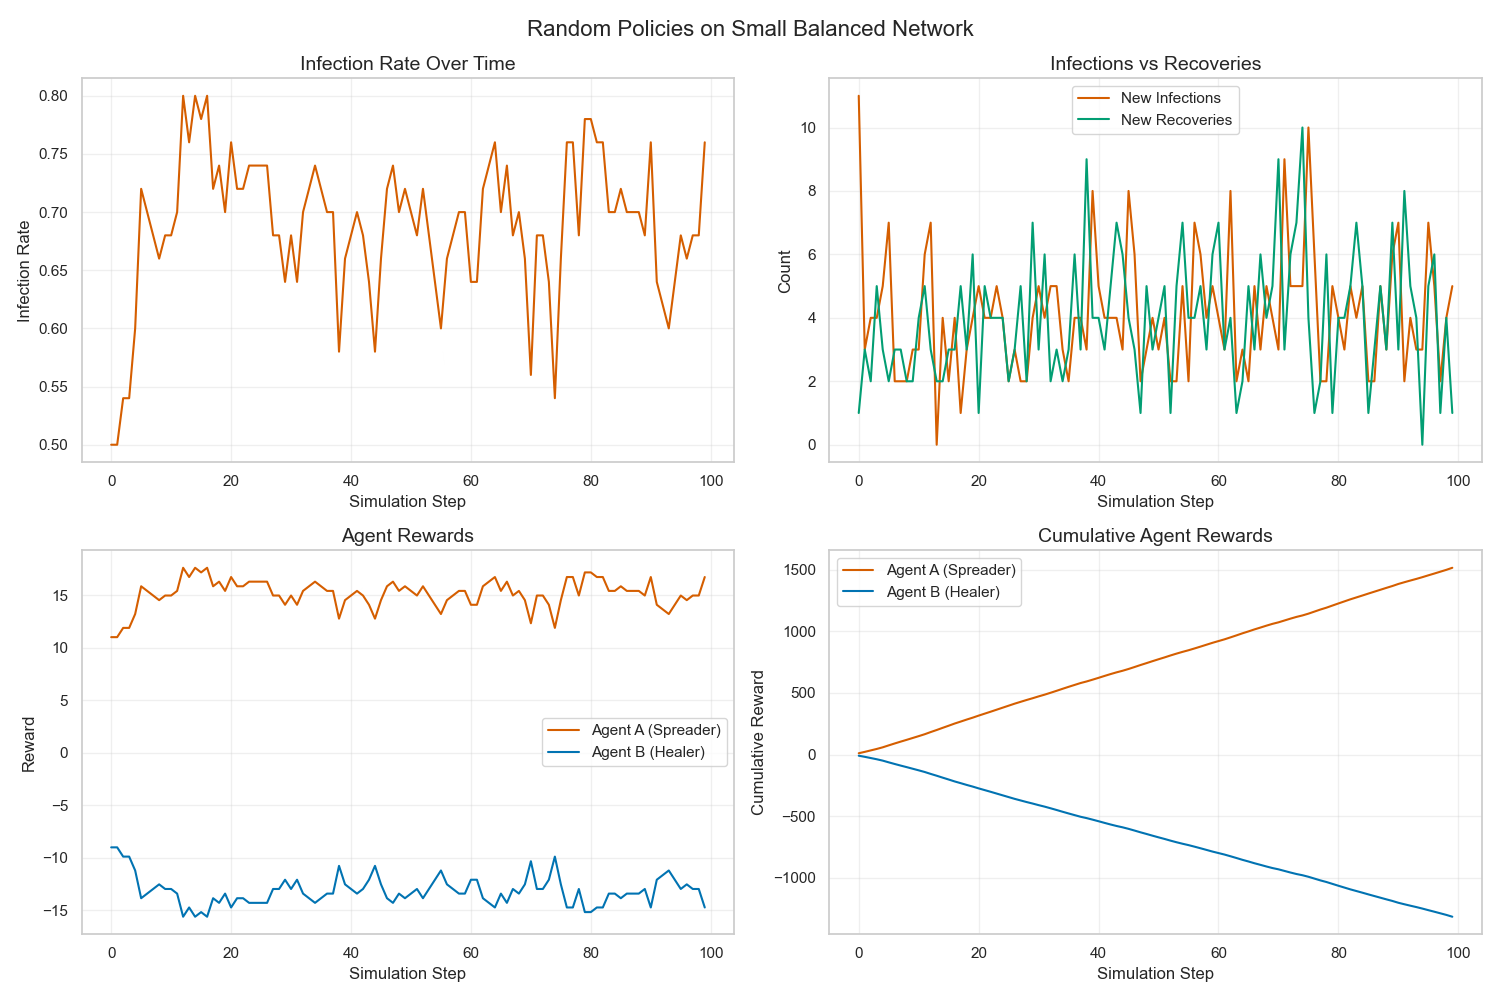
\includegraphics[width=\textwidth]{plots/random_policy_episode.png}
    \caption{Statistics summary for episode with random-choice policies.}
    \label{fig:random_episode}
\end{figure}
Figure \ref{fig:random_episode} suggests that random policies favor the spreading agent by a significant margin, with the spreading agent 
accumulating a significant amount of reward compared to the healing agent. 

\subsection{Training Dynamics}
Figure \ref{fig:training} shows the training progression for each network configuration. The infection rate and agent rewards over the course of training reveal how the agents learn to optimize their respective objectives.

\begin{figure}[h]
    \centering
    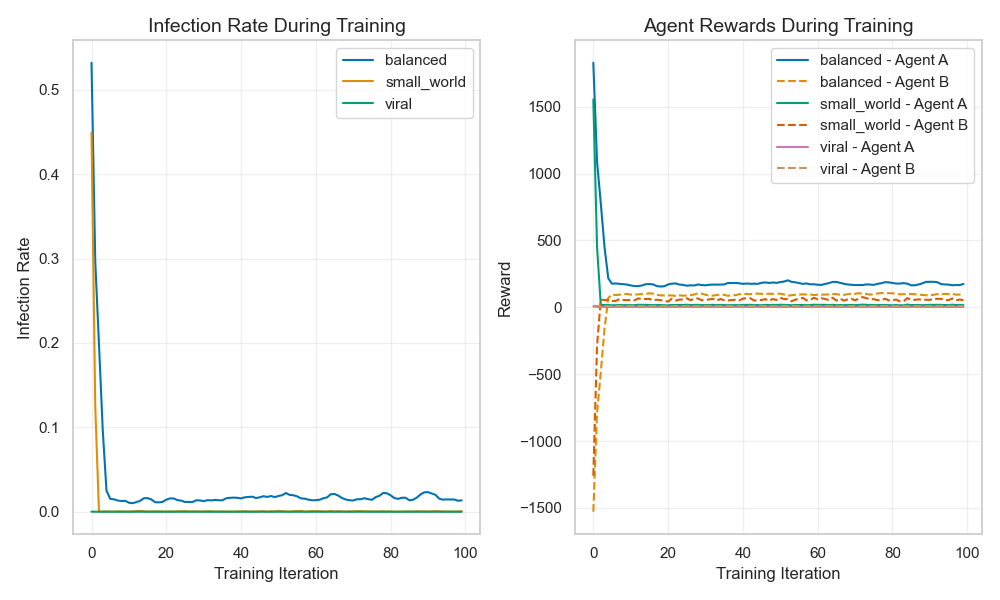
\includegraphics[width=\textwidth]{plots/training_comparison.png}
    \caption{Training progression across different network configurations. (a) Infection rate over training iterations. (b) Agent rewards over training iterations.}
    \label{fig:training}
\end{figure}

The glaring observation here is that once the Healing agent has learned how to contain the spread of infection, it is virtually impossible for the spreading agent to keep infection levels high, at least with our training environment parameters. 
This may indicate that our current model handicaps the spreading agent beyond what is reasonable. Nevertheless, 
we did not attempt to tweak training parameters much, 
mainly due to time and resources constraints. 
% \subsection{Network Structure Effects}

% The different network structures significantly influenced the dynamics of information spread and the effectiveness of agent strategies.

% \begin{figure}[H]
%     \centering
%     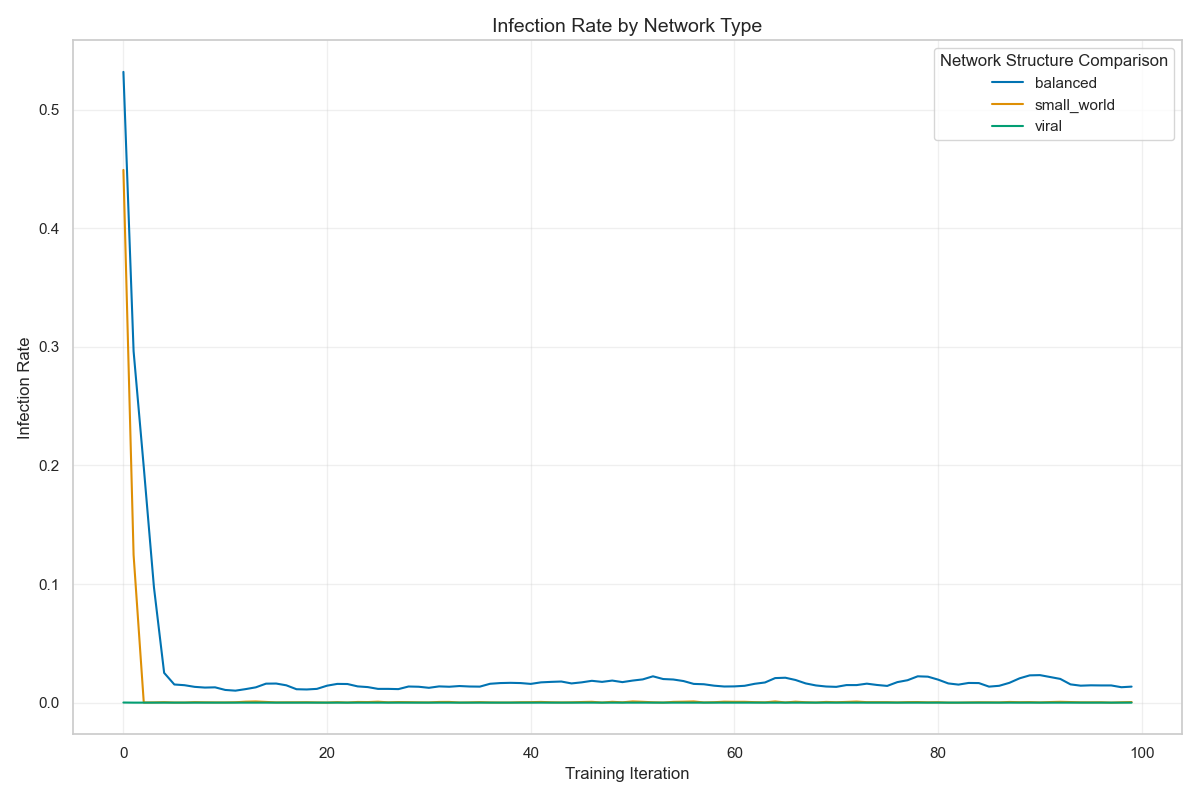
\includegraphics[width=0.8\textwidth]{plots/network_structure_effects.png}
%     \caption{Infection rate trajectories across different network types.}
%     \label{fig:network_structure}
% \end{figure}


\subsection{Agent Behavior Analysis}

Analysis of Agent B's behavior reveals interesting patterns in how it learns to optimally contain information spread. Figures 3-5 show Agent B's behavior patterns for each network configuration.

    \begin{figure}[h]
        \centering
        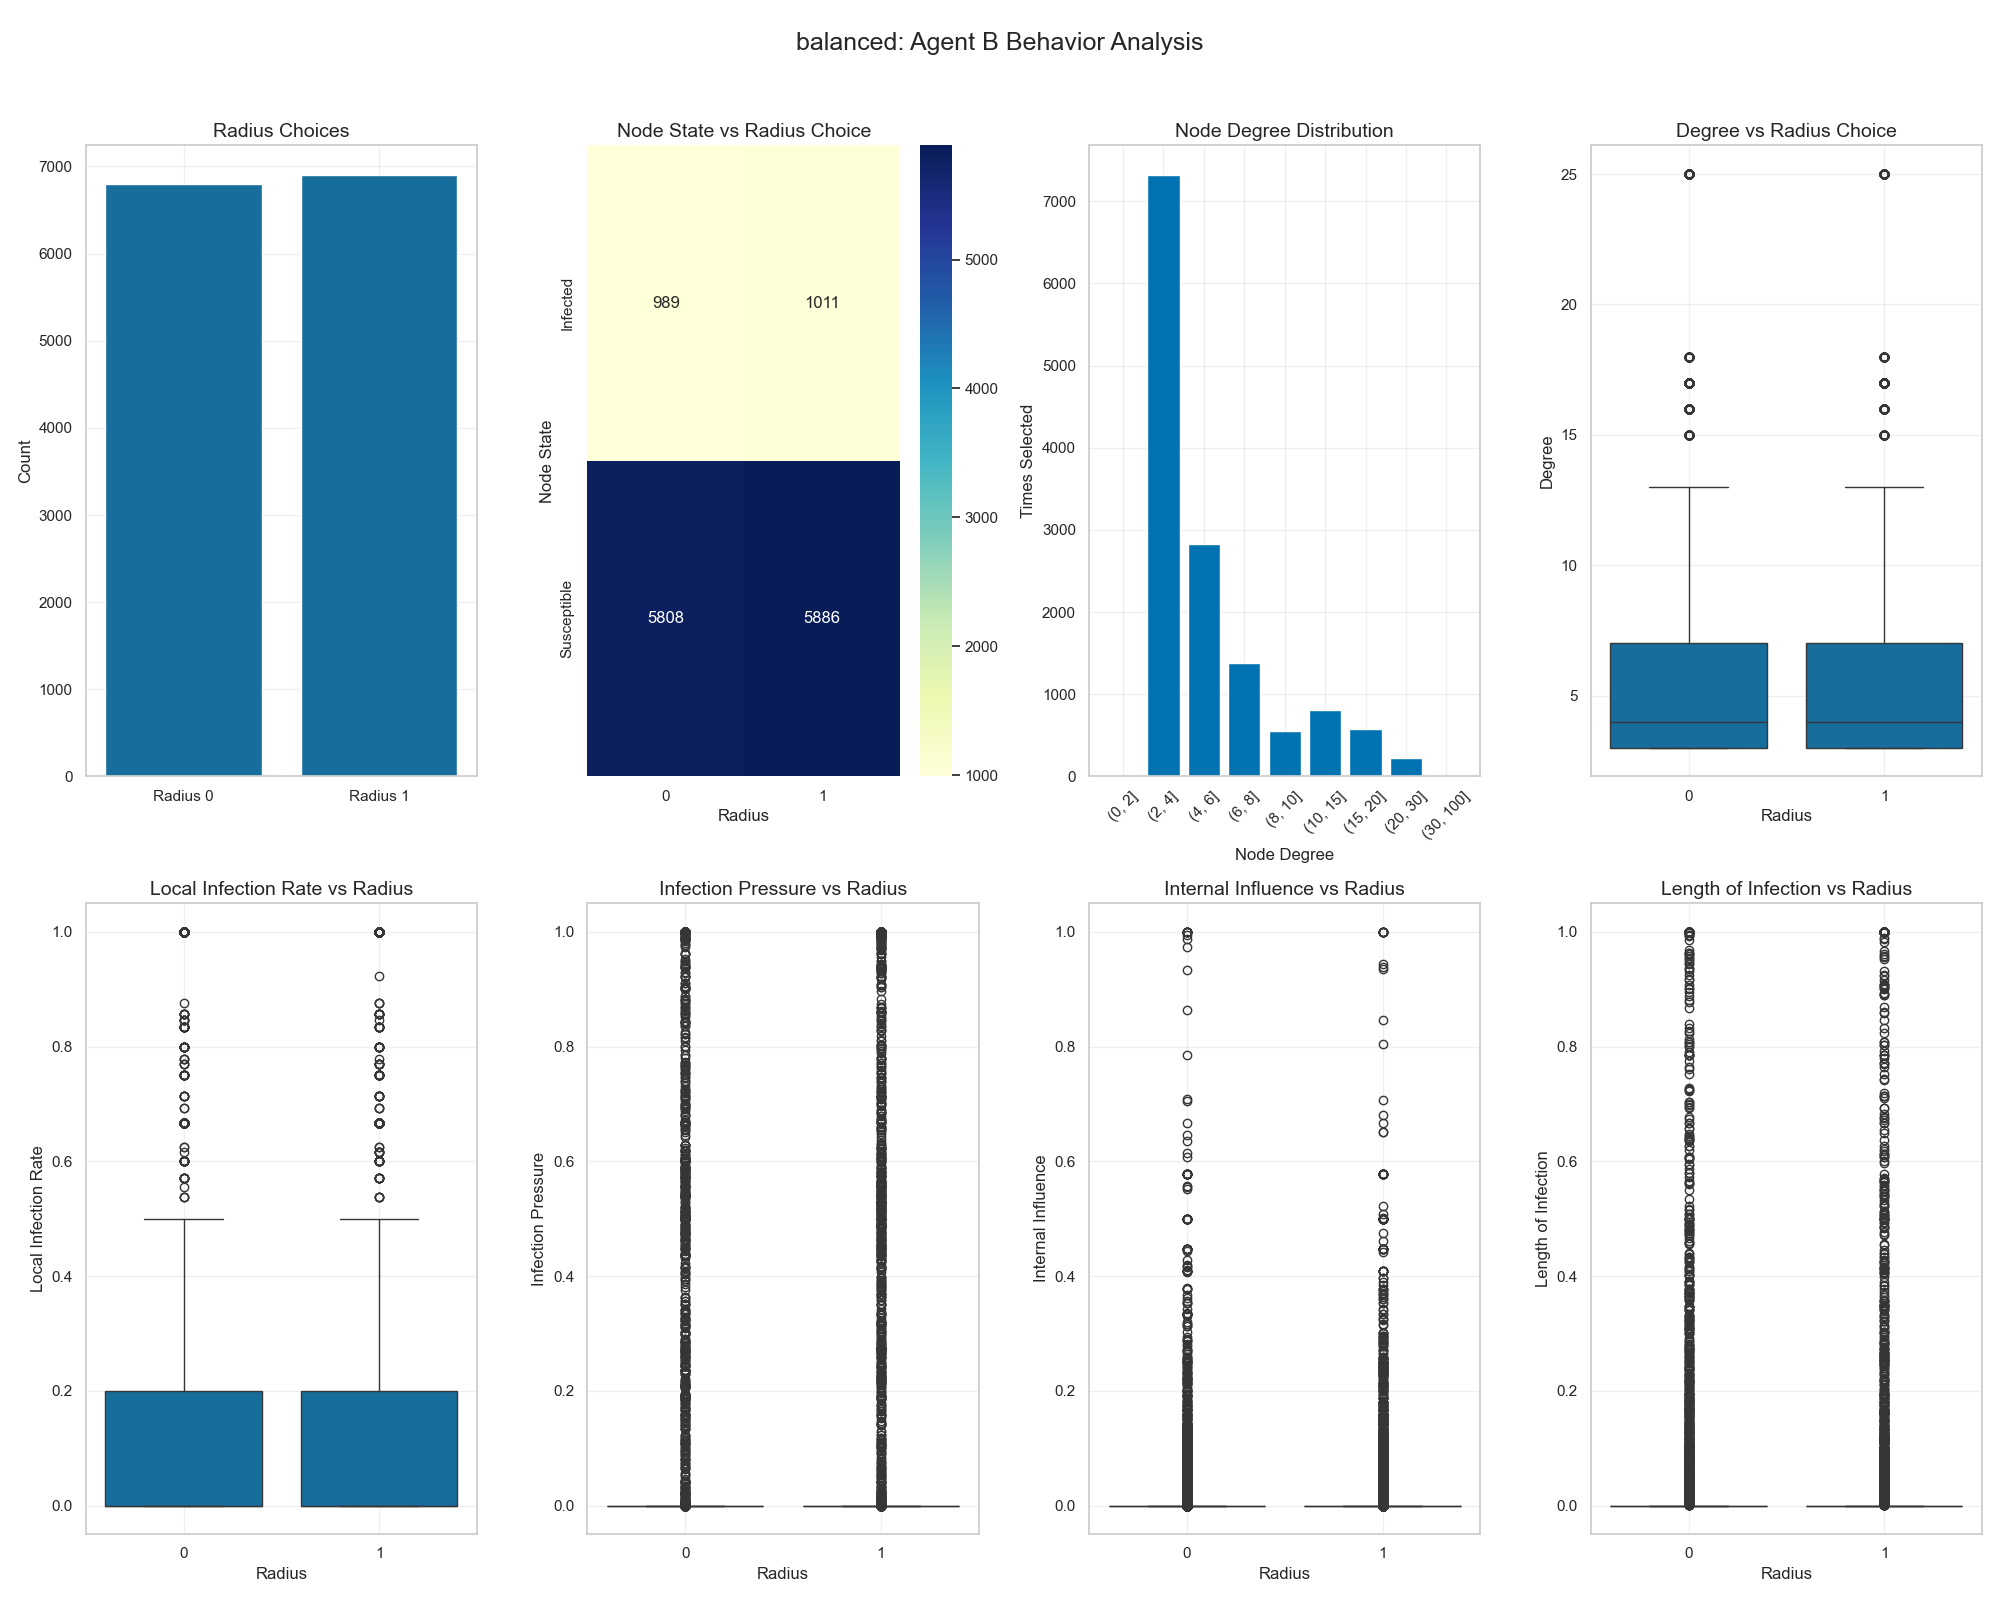
\includegraphics[width=\textwidth]{plots/balanced_agent_b_analysis.png}
        \caption{Agent B behavior in the balanced network configuration.}
        \label{fig:agent_b_balanced}
    \end{figure}
    \begin{figure}[h]
        \centering
        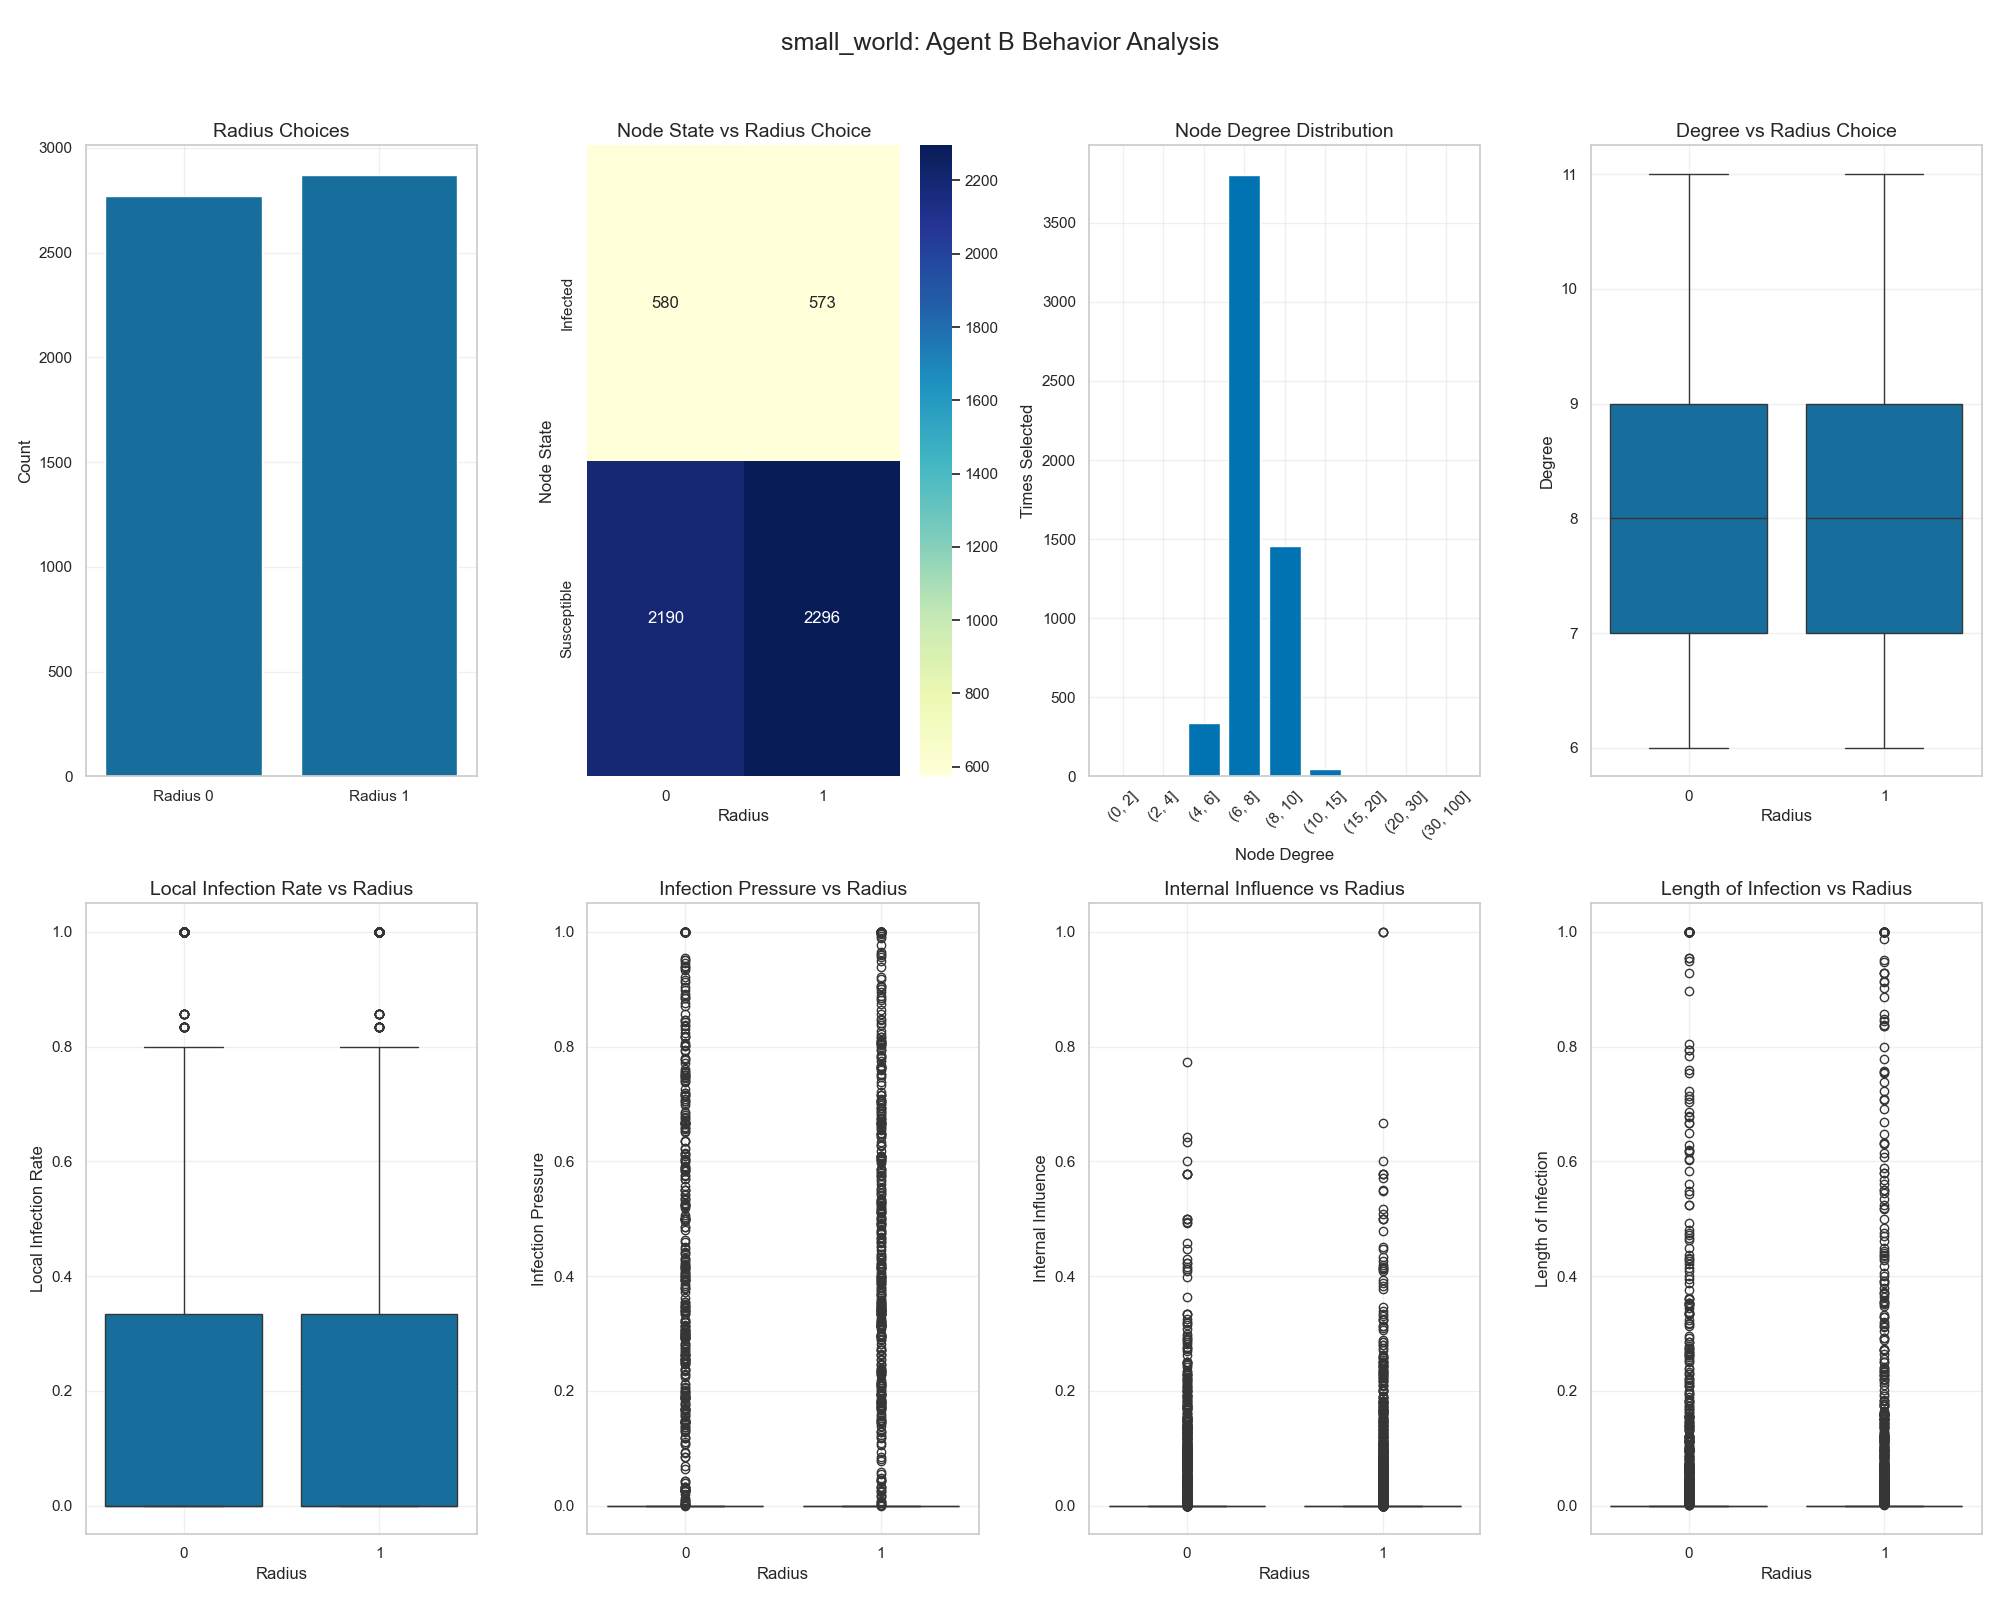
\includegraphics[width=\textwidth]{plots/small_world_agent_b_analysis.png}
        \caption{Agent B behavior in the small-world network configuration.}
        \label{fig:agent_b_small_world}
    \end{figure}
    \begin{figure}[h]
        \centering
        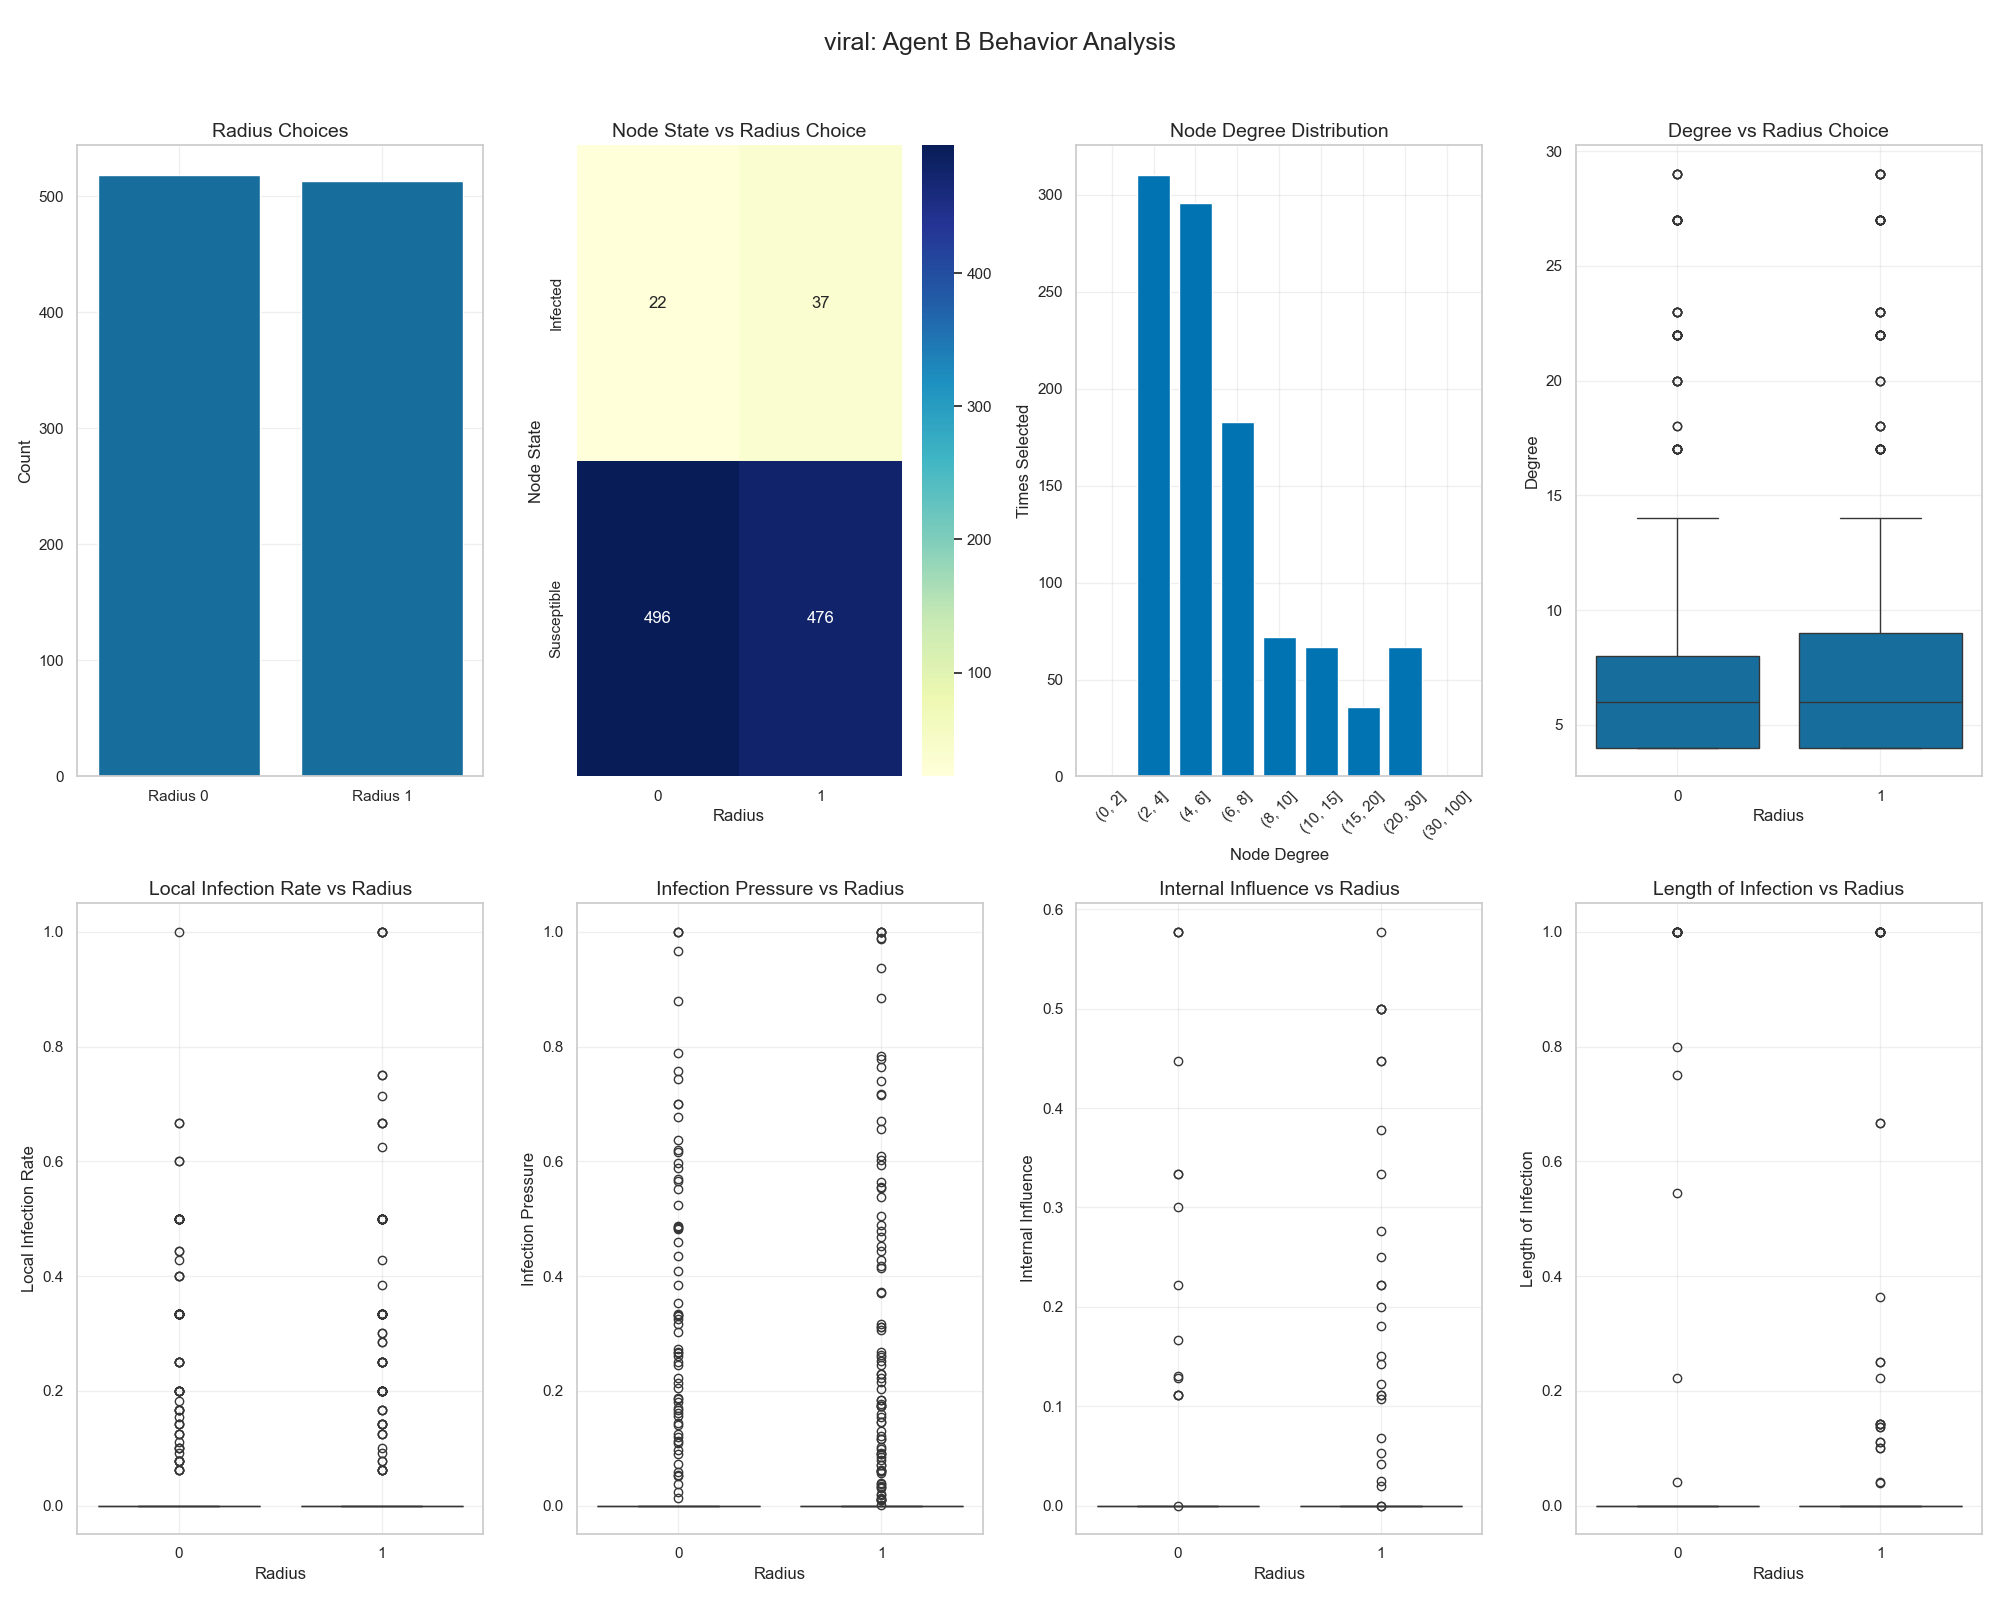
\includegraphics[width=\textwidth]{plots/viral_agent_b_analysis.png}
        \caption{Agent B behavior in the viral network configuration.}
        \label{fig:agent_b_viral}
    \end{figure}    

    \subsection{Baseline Comparison}
    We run an episode using our trained policies, to exemplify the effect of training on spread dynamics (Figure \ref{fig:viral_episode}). The side by side comparison shows a stark 
    constrast between the spread dynamics in both settings. 
    \begin{figure}[h]
        \centering
        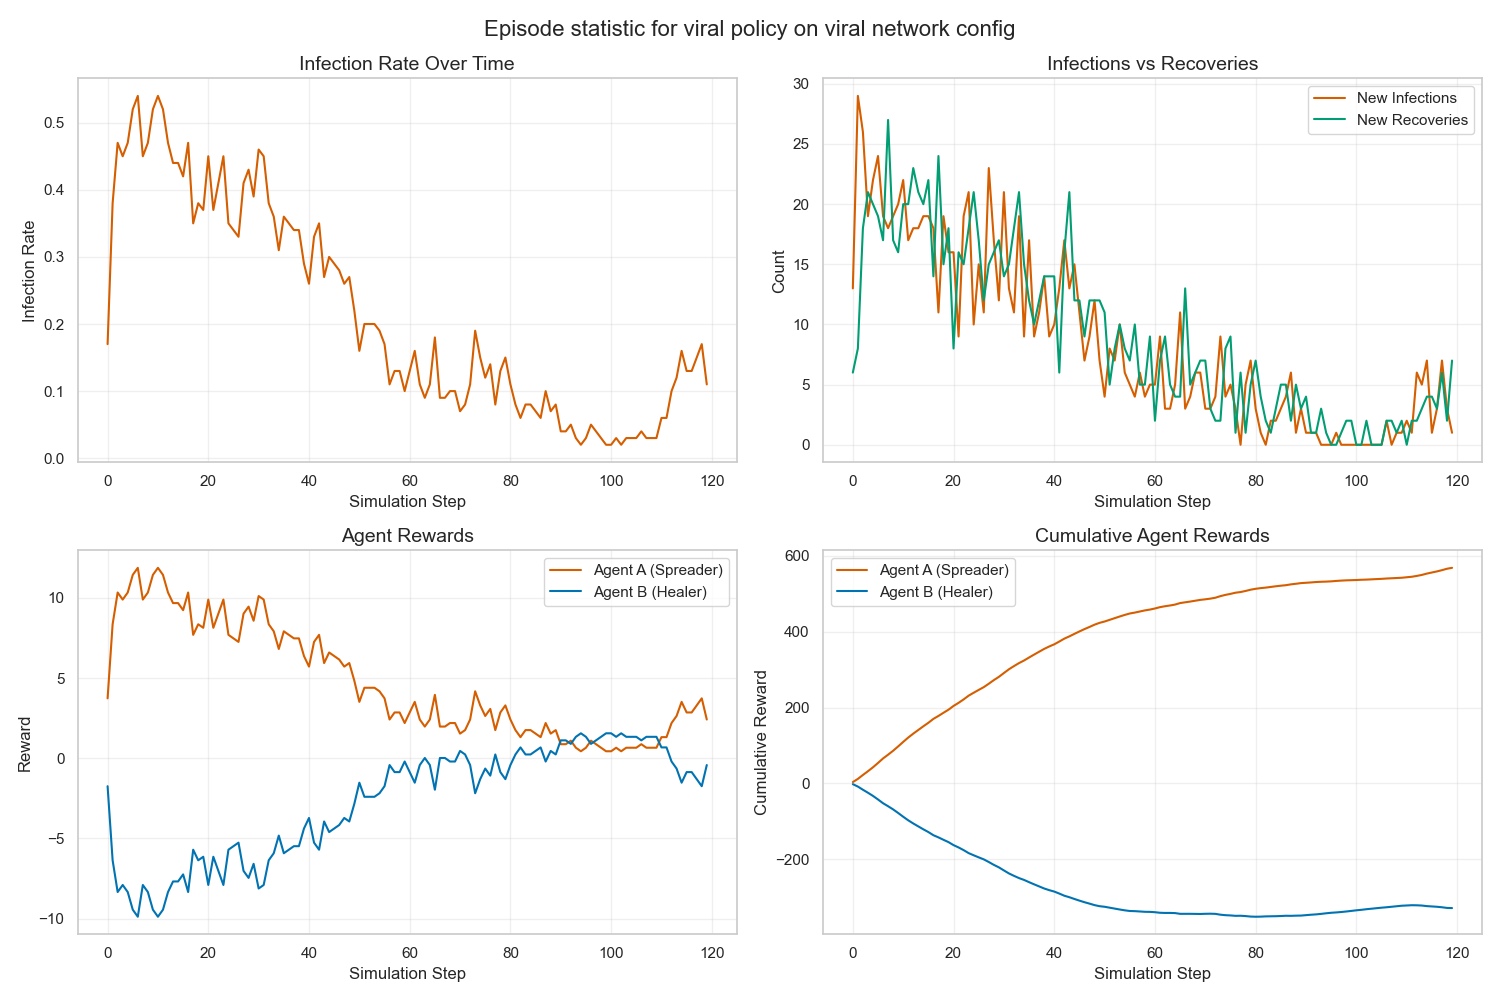
\includegraphics[width=\textwidth]{plots/viral_policy_episode_statistics.png}
        \caption{Episode statistics for viral policy on viral network configuration.}
        \label{fig:viral_episode}
    \end{figure}    

    \subsection{Parameter Sweep}
    We run a parameter sweep on intial infection/recovery probabilites 
    for various initial densities. As Figure \ref{fig:3d-Surface} shows, the most important parameter in our viral network configuration is not how fast the infection spreads, but how likely recovery is after infection. 
    \begin{figure}[!h]
        \centering
        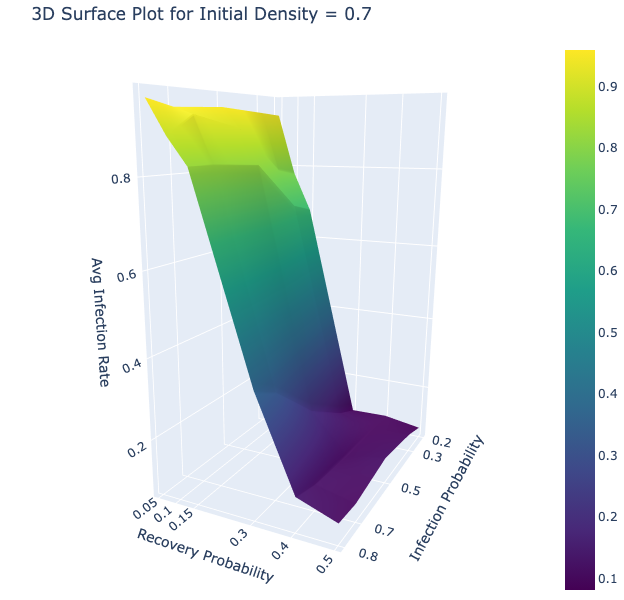
\includegraphics[width=\textwidth]{plots/sweep_3d.png}
        \caption{Surface plot for our parameter sweep.}
        \label{fig:3d-Surface}
    \end{figure}   

% \subsection{Parameter Sweep}
% The parameter sweep revealed how different combinations of infection probability, recovery probability, and initial infection density affect the dynamics of information spread and the effectiveness of agent strategies.

% \begin{figure}[H]
%     \centering
%     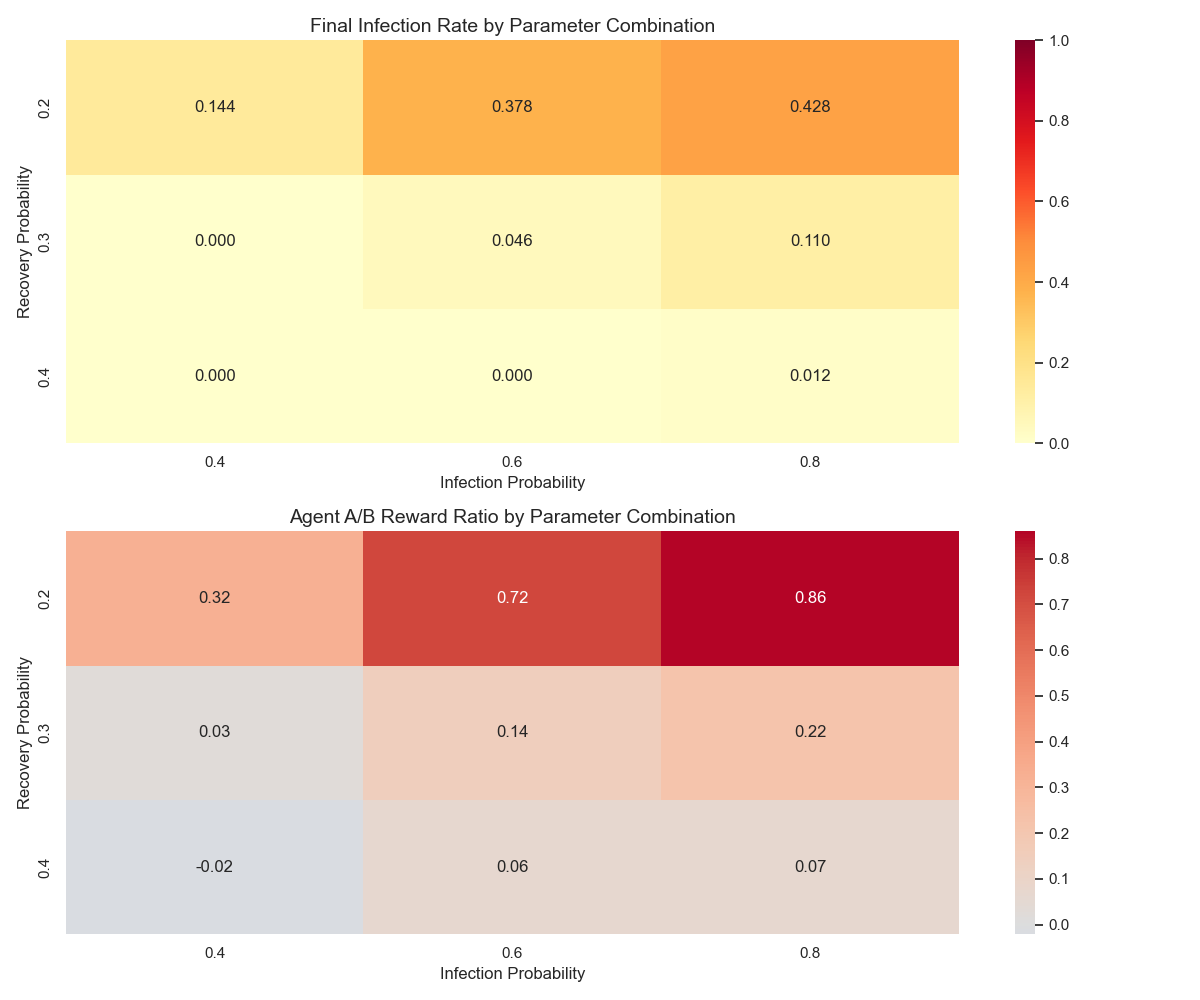
\includegraphics[width=0.8\textwidth]{plots/parameter_sweep_heatmap.png}
%     \caption{Parameter sweep results. (a) Final infection rate by parameter combination. (b) Agent reward ratio by parameter combination.}
%     \label{fig:parameter_sweep}
% \end{figure}
\section{Discussion}

\subsection{Interpretation of Results}


\subsection{Implications for Misinformation Management}

Our results have several implications for the management of misinformation in social networks, and are instrumental in 
partiall answering the questions posed at the start of this paper. 

\begin{enumerate}
    \item It appears that pre-emptive, individual intervention is, at the very least, as important as community-based interventions
    \item Under trained strategies, spreading agents struggle to keep infection rates above 10\%, unless recovery probability is low. 
    \item Denser networks are more conducive to the spread of misinformation, especially those with with more homogenous degrees across nodes. 
\end{enumerate}

These results suggest that a good way to mitigate information may be to ensure there are safeguards in place for recovery rates to never drop too low. Regretfully, we do not have the time to expand upon the corresponding tentative social policies that could mimick these results, as having a meaningful discussion thereof would require much more careful calibrating and statistical analysis on our part. 

\subsection{Limitations}
While our model provides valuable insights into the dynamics of information spread and containment, it has several limitations:

\begin{enumerate}
    \item Binary state representation: Our model uses a binary state representation (susceptible or infected), which may not capture the nuanced continuum of belief adoption in real social networks.
    
    \item Fixed network structure: Although we test different network topologies, each network's structure remains fixed throughout the simulation. In reality, social networks evolve over time as relationships form and dissolve.
    
    \item Limited agent capabilities: Our agents have a restricted set of actions available to them. Real-world actors engaging in information spread or containment may have a wider range of strategies at their disposal.
    
    \item Simplified diffusion mechanics: Our infection and recovery processes are simplified approximations of real-world information adoption and rejection processes.
    
    \item Scaling limitaitons: Our observation space 
    depends directly on the network's number of nodes, 
    making it impossible to transfer agent learning to networks whose size does not match the training network.
    
    \item Lack of spread model considerations: Our model does not implement echo chamber effects, which have the potential to change the resulting agent behaviors significantly. 
\end{enumerate}

\subsection{Future Directions}

Based on our findings and the limitations of our current model, we identify several promising directions for future research:

\begin{enumerate}
    \item Dynamic network structure: Extending the model to include dynamic network structure that evolves in response to information diffusion would more accurately reflect real-world social networks.
    
    \item More sophisticated state representation: Implementing a continuous or multi-level state representation could better capture the nuanced process of belief adoption.
    
    \item Additional agent capabilities: Expanding the action space of agents to include more diverse strategies, such as creating counter-narratives or strengthening community structures, could provide insights into more complex intervention strategies.
    
    \item Real-world validation: Validating model predictions against empirical data from real-world information diffusion events would strengthen the applicability of the findings.

    \item Implementing Graph Neural Networks: Using 
    a specialized learning architecture instead of a vanilla PPO algorithm will allow us to scale training 
    on small synthetic networks to larger, real-life social networks. The implementation of more Graph Attention Mechanisms could provde especially powerful. 
\end{enumerate}

\section{Conclusion}

In this paper, we presented a multi-agent reinforcement learning model for information spread and containment in social networks. Our model features two competing agents—a spreader and a healer—that learn to optimize their strategies for either maximizing or minimizing the spread of information. Through a series of experiments across different network configurations and parameter settings, we demonstrated how network structure, diffusion parameters, and agent capabilities influence the dynamics of information spread.
Our results showed that pre-emptive intervention is often more effective in networks with low infection rates. These patterns may generalize to different initial settings, but to answer this would require analyzing the Healing agent's actions on a sweep of initial infection rates. These findings contribute to our understanding of how strategic interventions can influence information diffusion processes in social networks and provide insights for the development of more effective approaches to misinformation management.


By combining concepts from network science, epidemic modeling, and reinforcement learning, our work offers a novel perspective on the strategic dynamics of information spread and containment. As social media platforms continue to play a central role in information dissemination, models like ours can help inform the design of interventions that promote the spread of accurate information while limiting the reach of harmful misinformation.

\bibliographystyle{apalike}
\bibliography{references}

\end{document}